\documentclass[]{article}

\usepackage{
	amsmath, 
	amssymb,
	float,
	graphicx,
	bera,
	parskip
}

\usepackage[
backend=biber, 
style=authoryear,
citestyle=apa, 
sorting=ynt]{biblatex}

\graphicspath{{Images/}}

\title{Assignment 4}
\author{
	Daniel Bok \\
	ESD \\
	1001049 \\
	daniel\_bok@mymail.sutd.edu.sg 
	\and
	Wong Yan Yee\\ 
	ISTD \\
	1001212 \\
	yanyee\_wong@mymail.sutd.edu.sg
	\and
	Clement Tan \\
	ESD \\
	1000948 \\
	clement\_tan@mymail.sutd.edu.sg
}
\date{\today}

\newcommand{\e}{&=}

\begin{document}
	
\maketitle

\newpage
\section*{Exercise 1: Computation of $C$ and $L$}

\subsection*{Part A}
\begin{figure}[H]
	\centering
	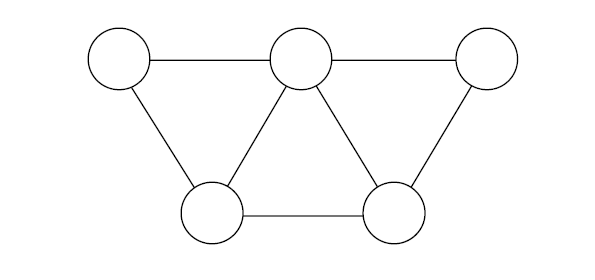
\includegraphics[width=\linewidth]{Graph-1.png}
	\caption{Graph 1}
	\label{fig:graph-1}
\end{figure}

\begin{align*}
\text{Connected Triples} \e 5 + 4 + 3 + 2 \\
	\e 14 \\
\text{Triangles} \e 3 \\
C \e \frac{3}{14} \\
L \e 2
\end{align*}

\subsection*{Part B}
\begin{figure}[H]
	\centering
	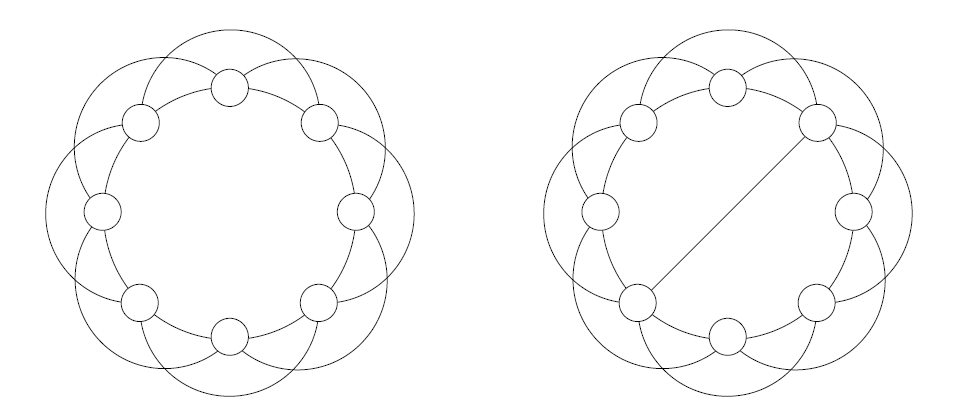
\includegraphics[width=\linewidth]{Graph-2.png}
	\caption{Graph 2}
	\label{fig:graph-2}
\end{figure}

We take $n = 8$ and $c = 4$ in both graphs seen in Figure \ref{fig:graph-2}.
\begin{align*}
\begin{split}
\text{Connected Triples} \e n\binom{c}{2} = n\binom{4}{2} = 6n \\
\text{Triangles} \e n\binom{\frac{c}{2}}{2} = n\binom{2}{2} = n\\
C \e \frac{n}{\frac{6}{3}n} = \frac{1}{2} \\
L \e \frac{n}{c} = \frac{8}{4} = 2
\end{split} 
\begin{split}
\text{Connected Triples} \e \binom{4}{2}n + 8 = 56 \\
\text{Triangles} \e \binom{2}{2}n + 2 = 10 \\
C \e \frac{10}{\frac{56}{3}} = \frac{15}{28} \\
L \e 2
\end{split}
\end{align*}

\newpage
\section*{Kleinberg Model}

\subsection*{Part B}
\begin{figure}[H]
	\centering
	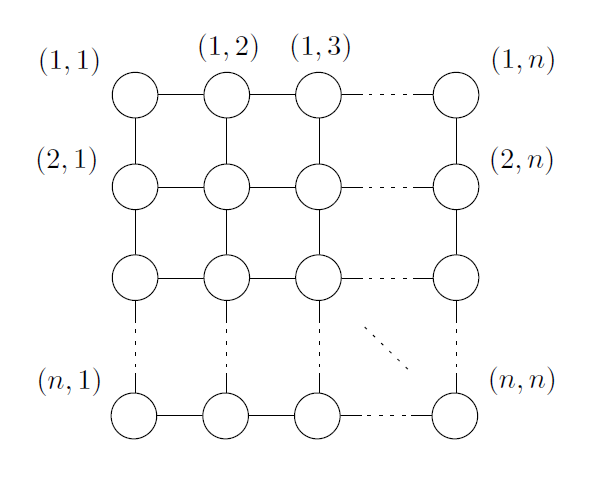
\includegraphics[width=\linewidth]{Graph-3.png}
	\caption{2-Dimensional Lattice (Kleinberg Model)}
	\label{fig:graph-3}
\end{figure}

\subsection*{Part A}

We assume the question that the distance, $D$, implies the minimum steps required to get from node (1, 1) to any node. Therefore, $D=3$ will not include path such as
\[
(1, 1) \rightarrow (1, 2) \rightarrow (2, 2) \rightarrow (2, 1)
\]
because (2, 1) can be travelled with a minimum of 1 step. Given this assumption, the general formula is given by:
\begin{align*}
\text{Number of nodes given distance} \e 
\begin{cases}
	D + 1 		& 1 \leq D \leq n - 1\\
	2n - D - 1	& n \leq D \leq 2(n - 1)
\end{cases}
\end{align*}

Assuming $n > 3$ as seen from Figure \ref{fig:graph-3}, with the general formula, the number of nodes given distance are
\begin{align*}
D = 1  \rightarrow 2 \\ 
D = 2  \rightarrow 3 \\
D = 3  \rightarrow 4
\end{align*}

\subsection*{Part B}

We let $S(\cdot)$ denote the size function
\begin{align*}
S(B_j) \e 1 + \sum_{i = 1}^{2^j} (i + 1) \\
	\e 1 + 2^j + \frac{ 2^j (2^j + 1)}{2} 
\end{align*}

\subsection*{Part C}

Let the size of $R_j$ be denoted by $S(R_j)$. The exact size of $R_j$ is thus given by:
\begin{align*}
S(R_j) \e B_j - B_{j-1} \\
	\e 	2^j + 1 + \frac{2^j(2^j + 1)}{2} 
		- \left( 2^{j-1} + 1 + \frac{2^{j - 1}(2^{j - 1} + 1)}{2} \right) \\
	\e 2^j + 2^{2j - 1} + 2^{j - 1} - 2^{j - 1} - 2^{2j - 3} - 2^{j - 2} \\
	\e 2^j - 2^{j - 2} + 2^{2j - 1} - 2^{2j - 3} \\
	\e \frac{3}{4} \left( 2^j + 2^{2j - 1} \right) 
\end{align*}

The lower bound is thus given by $\frac{3}{4} \cdot 2^{2j-1} = 3 \cdot 2^{2j-3}$

\subsection*{Part D}

We take $\nu$ to be a node at the outermost boundary of $R_j$ and Node (1, 1) to be $\mu$. Given $\alpha = 2$, the probability of a random link between $\mu$ and $\nu$ is given by
\begin{align*}
Pr(\mu \leftrightarrow \nu) &\geq \frac{r^{-\alpha}}{4 \ln (6n)} \\
	&\geq \frac{2^{-2j}}{4 \ln (6n)}
\end{align*}

From Part C, since there are $3 \cdot 2^{2j-3}$ number of nodes in $R_j$, we get the lower bound for $\nu \exists R_j$ as
\begin{align*}
Pr(\mu \leftrightarrow \nu \exists R_j) &\geq 
	3 \cdot 2^{2j-3} \cdot \frac{2^{-2j}}{4 \ln (6n)} \tag{1} \label{eqn:1}\\
&\geq \frac{3}{32 \ln (6n)}
\end{align*}

No, the value does not depend on $j$.

\subsection*{Part E}

When $\alpha = 1$ or $\alpha=3$, the probability of the random connection will depend on  $j$ as we will not be able to take out the $j$ term from Equation \eqref{eqn:1}.

\newpage
\section*{Congestion Prices}

\subsection*{Part 1}

At equilibrium,
\begin{align*}
A  - cn \e 0 \\
n_o \e \frac{A}{c}
\end{align*}

\subsection*{Part 2}

We assume the social planner intends to maximize the utility for the all the theatre goers. His objective function is thus given by:
\begin{align*}
\max & \sum_{i=1}^{n} A - cn \\
	& An - cn^2
\end{align*}
At optimal
\begin{align*}
\frac{d}{dn} An - cn^2 \e 0 \\
A - 2cn \e 0 \\
n_s \e \frac{A}{2c} = \frac{1}{2} n_o
\end{align*}

At optimal $n_s = \frac{1}{2} n_o$, there would be 2 times more spectators than is socially optimal. Therefore, there is tragedy of the commons as spectators consume more seats than optimal.

\subsection*{Part 3}

We assume the social planner charges a price, $p$. The utility of each spectator would then be $A - cn - p$. At equilibrium,
\begin{align*}
A - cn - p \e 0 \\
n_{o} \e \frac{A - p}{c}
\end{align*}

For $n_o = n_s$,
\begin{align*}
\frac{A - p}{c} \e \frac{A}{2c} \\
p \e \frac{1}{2} A
\end{align*}

\subsection*{Part 4}

We denote by $U_i$ the utility of participant $i$ consuming one unit of movie. The net benefit accrued by a single participant will then be
\begin{align*}
U_i \e A - cn_s - p + \frac{n_sp}{n} \\
	\e A - cn_s - p \cdot \left( 1 - \frac{n_s}{n} \right)
\end{align*}
Where $n_s$ stands for the number of spectators in the theatre in the social optimal and $n$ stands for the population size (of spectators).

\newpage
\section*{Usage Prices}

\subsection*{Part 1}

At equilibrium, demand equals supply
\begin{align*}
x_1 + x_2 = C
\end{align*}
We denote the price to clear the market as $P$.
\begin{align*}
U_1(x_1) \e a \log x_1 - P \cdot x_1 \\
\frac{dU_1(x_1)}{dx_1} \e \frac{a}{x_1} - P \\ \\
U_2(x_2) \e b \log x_2 - P \cdot x_2 \\
\frac{dU_2(x_2)}{dx_2} \e \frac{b}{x_2} - P 
\end{align*}
where $U_i(x_i)$ denotes the utility gained by user $i$ consuming $x_i$ units of bandwidth and $\frac{dU_i(x_i)}{dx_i}$ represents the marginal utility of user $i$.

We note that at equilibrium, the marginal utility rate must be similar. Thus we obtain the bandwidth allocation,
\begin{align*}
\frac{a}{x_1} - P \e \frac{b}{x_2} - P \\
x_1 \e \frac{a x_2}{b} \\
C \e x_2 (1 + \frac{a}{b}) \\
x_2 \e C \cdot \frac{b}{a + b} \\
x_1 \e C \cdot \frac{a}{a + b}
\end{align*}

Rewriting the marginal utility functions for each player and setting them to 0, we obtain the price
\begin{gather*}
b \cdot \frac{a + b}{C b} - P = 0 \\
P = \frac{a + b}{C}
\end{gather*}

\subsection*{Part 2}

With infinite capacity, the bandwidth will be sold at marginal cost. Thus, $P = c$. Thus, the utility functions will be given by
\begin{align*}
U_1(x_1) \e a \log x_1 - cx_1 \\
\frac{dU_1(x_1)}{dx_1} \e \frac{a}{x_1} - c = 0 \\ 
x_1 \e \frac{a}{c} \\ \\
U_2(x_2) \e b \log x_2 - c \cdot x_2 \\
\frac{dU_2(x_2)}{dx_2} \e \frac{b}{x_2} - c = 0 \\
x_2 \e \frac{b}{c} 
\end{align*}

\subsection*{Part 3}

\subsubsection*{Case 1}

With a capacity of $C$, we have a bandwidth constraint given by
\begin{align*}
\sum_{i=1}^{n} x_n \e C \\
nx \e C \quad \text{(gross consumption)} \\
x_i \e \frac{C}{n}  \quad \text{(individual consumption)}
\end{align*}
Given a price of $P$, the marginal utility for user $i$ is given by
\begin{align*}
U_i(x_i) \e a \log x_i - P_1x_i \\
\frac{dU_i(x_i)}{dx_i} \e \frac{a}{x_i} - P_1
\end{align*}
At equilibrium, supply equals demand. The marginal utility is thus 0. The price to clear this market will then be given by
\begin{align*}
\frac{a}{x_i} - P_1 \e 0 \\
P_1 \e \frac{a}{x_i} \\
P_1 \e \frac{an}{C}
\end{align*} 

\subsubsection*{Case 2}

With an infinite capacity, the price at which bandwidth is sold will be equal to the marginal cost ($P_2 = c$) since the network will only supply up to the point where it does not make a loss.

\subsubsection*{Comments}

We see the difference in prices, where $P_1 \geq P_2$, because capacity is limited in Case 1. This limitation causes the bandwidth supplier to charge higher than the marginal cost to limit the amount that the $n$ users want to consume individually, thus tapering the demand.

We do not assume the case where $P_1 < c$. In such a case, the supplier can always reduce the capacity (supply) or just charge at marginal cost (equivalent of reducing supply).

\subsection*{Part 4}

The network operator can charge a fixed fee $\beta$ on top of the usage fee $P = c$. Since the operator does not know the utility (and thus the demand functions) of the users, he would not be able to charge an optimal price.

For example, he may charge too expensive $\beta$ and risk losing the weak user as $\beta > CS_A$. $CS_A$ represents the consumer surplus of user $A$.

\subsection*{Part 5}

\begin{gather*}
x_a + x_b = C \\
\text{(From Part 1)} \\
P = \frac{a + b}{C} \\
x_a = \frac{Ca}{a + b} \quad x_b = \frac{Cb}{a + b}
\end{gather*}

\begin{align*}
\begin{split}
CS_A \e a \log x_a - P \cdot x_a \\
\end{split}
&\ 
\begin{split}
CS_B \e b \log x_b - P \cdot x_b \\
\end{split}
\end{align*}

\begin{description}
\item[Case 1] Both players participate. Fixed fee equals the consumer surplus of the weaker player. $\beta = CS_A$

\begin{align*}
\beta_1 \e a \log \frac{Ca}{a + b} - \frac{a + b}{C} \cdot \frac{Ca}{a + b} \\
\e a \left( \log \frac{Ca}{a + b} \right) - a
\end{align*}

The profit is given by
\begin{align*}
\pi_1 \e 2 \beta_1 + P \cdot x_1 + P \cdot x_2 \\
\e 2 \beta_1 + \frac{a + b}{C} \left( \frac{Ca}{a + b} + \frac{Cb}{a + b} \right) \\
\e 2 \beta_1 + a + b \\
\e 2a \left( \log \frac{Ca}{a + b} \right) - a + b
\end{align*}

\item[Case 2] Fixed fee too high, thus only the stronger player participates.

\begin{align*}
\beta_2 \e b \log \left( \frac{Cb}{a + b} \right) - \frac{a + b}{C} \cdot \frac{Cb}{a + b} \\
\e b \left( \log \frac{Cb}{a + b} \right) - b
\end{align*}

The profit is given by
\begin{align*}
\pi_2 \e \beta_2 + P \cdot x_2 \\
\e b \left( \log \frac{Cb}{a + b} \right) - b + \frac{a + b}{C} \left( \frac{Cb}{a + b} \right) \\
\e b \left( \log \frac{Cb}{a + b} \right)
\end{align*}
\end{description}

For large values of $C$, the network operator will choose to use the option which gives him the higher profit. He would thus choose to set a fixed fee of $\beta_1$ if
\begin{align*}
\pi_1 &\geq \pi_2 \\
2a \left( \log \frac{Ca}{a + b} \right) - a + b &\geq b \left( \log \frac{Cb}{a + b} \right) \\
\approx a \left( 2 \log C - 1 \right) &\geq b \left( \log C - 1 \right)
\approx 2a &\geq b
\end{align*}

Otherwise, if $2a < b$, he would choose $\beta_2$. In all cases, User B will benefit more. In Case 1, User B will still have a greater consumer surplus than User A. In Case 2, since User A is not consuming anything, User B will have a benefit that is $\epsilon$ greater than User A. 

\end{document}
